\section{Introduction and Concepts}
Traditional Networking Architecture is divided into different independent planes on each device, depending on the layer.
\begin{table}[h]
	\begin{tabular}{p{0.1\textwidth}|p{0.25\textwidth}|p{0.35\textwidth}|p{0.3\textwidth}}
		. & Control Plane & Data Plane & Management Plane \\ 
		\hline
		Layer 2 & Spanning Tree Overlays (VLANs) & Forward \emph{Ethernet Frames} & Configuration \\ \hline
		Layer 3 & Routing Protocols Overlays (MPLS) & Forward \emph{IP Packets} & Configuration 
	\end{tabular}
\end{table}

\noindent
This results in some drawbacks such as:
\begin{itemize}
	\item Limited decision making ``intelligence''
	\item Difficult administration
	\item Missing overall analytics
\end{itemize}

\subsection{Vision of SDN}
\begin{itemize}
	\item Hardware: cheaper
	\item Software: features frequent releases, decoupled from hardware
	\item Functionality: driven by software and controller. Aiming for a programmable network
	\item Simplicity: from manual to automated, from box centric to network wide, from provisioning in months to provisioning in hours
	\item Innovations: from closed systems to open and programmable
\end{itemize}

\noindent
\emph{Virtualization of Computing needs virtualization of Network!}

\subsection{SDN Devices}
All Information from FIB to Config can be updated via API calls (support depending: RESTCONF, NETCONF, \ldots)
\\
\\
\noindent
White box switches 
\begin{itemize}
	\item support OpenFlow 1.3
	\item Third Party OS Support
\end{itemize}

\noindent
White box OS
\begin{itemize}
	\item Open Compute Project OCP
	\item Pica8
	\item Nvidia Cumulus Linuz
	\item opennetlinux.org
	\item fboss
\end{itemize}



\subsection{SDN Approaches}
Different levels of abstraction can be applied to the topology, resulting in mainly three different SDN approaches. 

\begin{figure}[h]
	\centering
	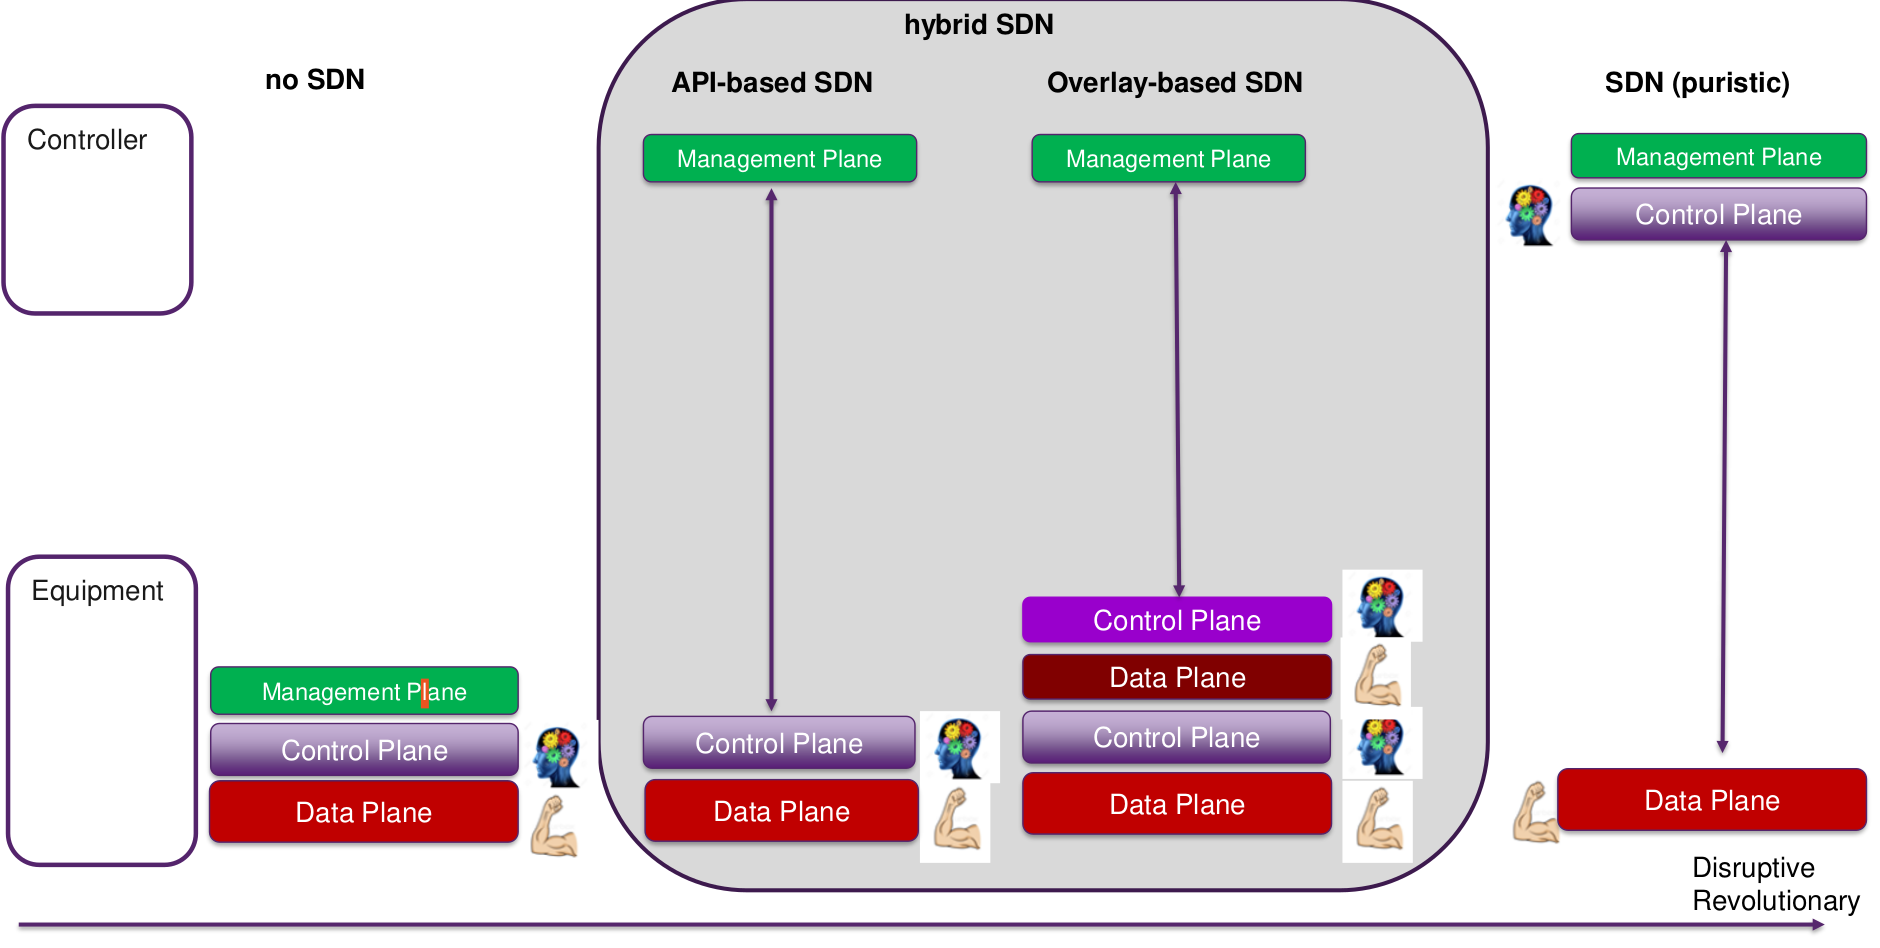
\includegraphics[width=\textwidth]{sdn-approaches}
	\caption{Different abstraction levels}
\end{figure}

\subsubsection{Pure SDN}
Academic approach.
Only Data Plane on each device. 
Management and Control Plane centralized, resulting in full decoupling. 
OpenFlow Protocol distributes information, unknown Packets are sent to controller. 
Flow table is used for forwarding decisions. 

\begin{figure}[h]
	\centering
	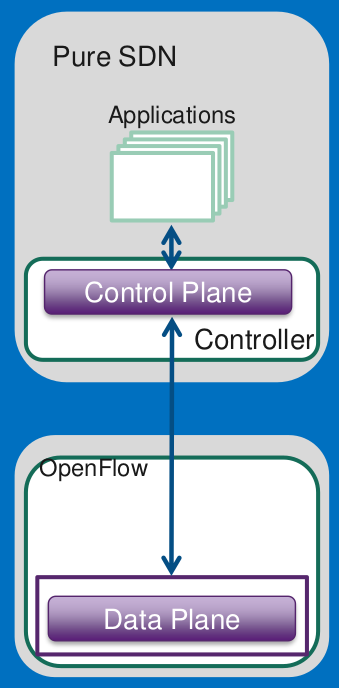
\includegraphics[width=3cm]{pure-sdn}
	\caption{Pure SDN}
\end{figure}
\begin{figure}[h]
	\centering
	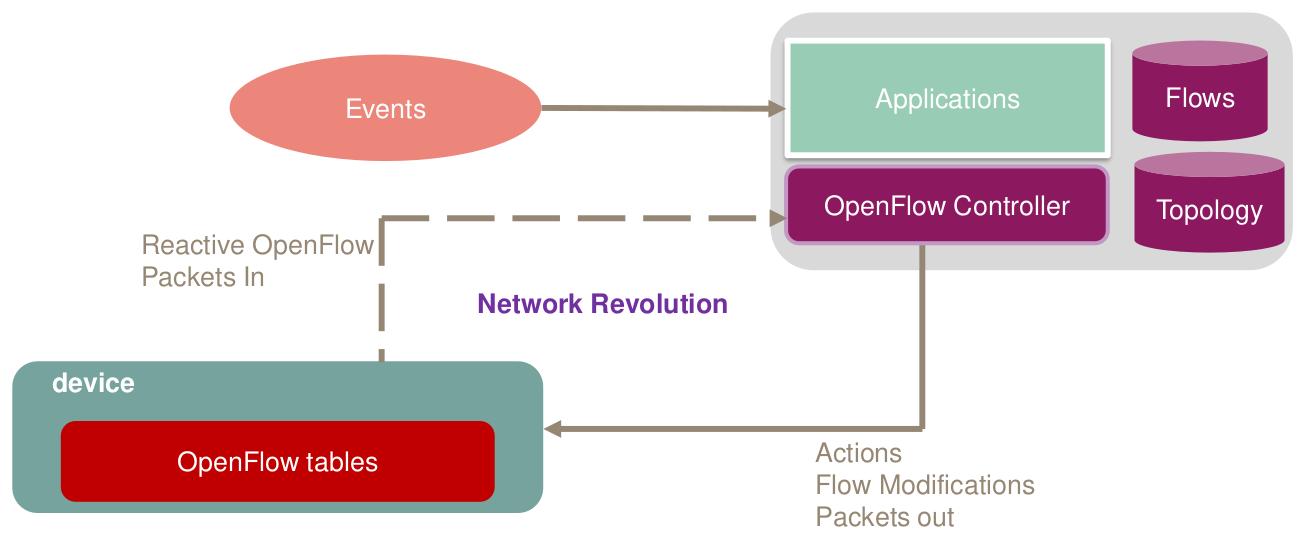
\includegraphics[width=10cm]{approach-pure-sdn}
	\caption{Pure SDN}
\end{figure}

\noindent
\textbf{Positive}
\begin{itemize}
	\item Independent evolution and development 
	\begin{itemize}\item software control of the network can evolve independently from hardware \end{itemize}
	\item control from high-level software program 
	\begin{itemize}\item debug/check behaviour more easily 
	\item testing/troubleshooting\end{itemize} 
\end{itemize}

\noindent
\textbf{Negative}
\begin{itemize}
	\item controller could be single point of failure 
	\item no topology change without controller 
	\item migration
	\item high risk
\end{itemize} 


\subsubsection{Hybrid SDN, API based}
Data and Control Plane on each device, Management Plane centralized. Similar to snmp, ssh scripts. 

\begin{figure}[h]
	\centering
	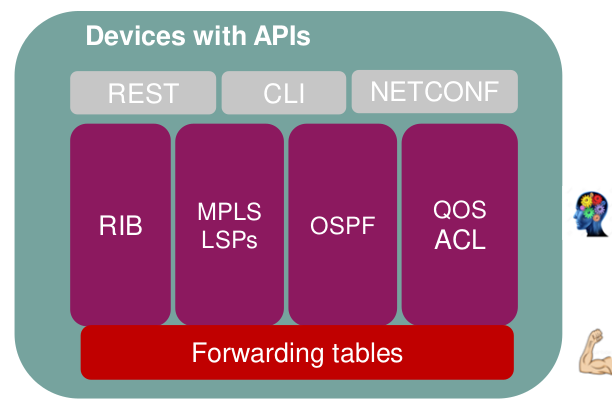
\includegraphics[width=5cm]{devices-api}
	\caption{Hybrid: API based SDN}
\end{figure}

\begin{figure}[h]
	\centering
	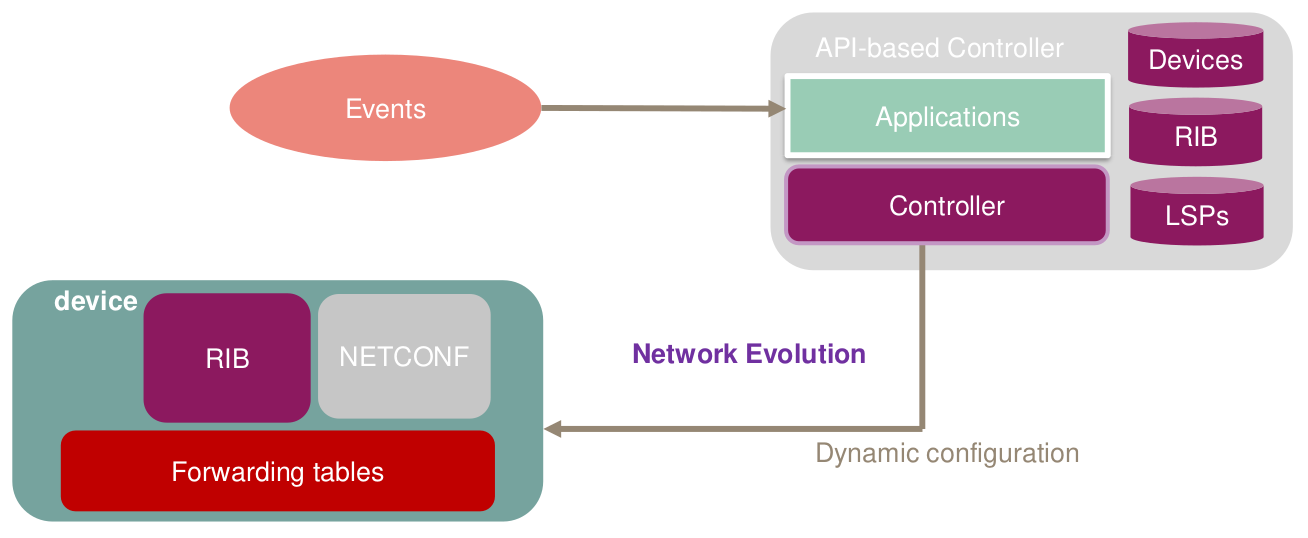
\includegraphics[width=10cm]{approach-api-sdn}
	\caption{Hybrid: API based SDN}
\end{figure}

\noindent
\textbf{Positive}
\begin{itemize}
	\item Faster provisioning of new customers and services 
    \item Low impact in case of controller loss: 
	\begin{itemize}
        \item Provisioning delayed
        \item Visibility loss 
		\item Equivalent to any orchestration system failure 
	\end{itemize}
	\item Network partitioning: low impact 
	\item Increased flexibility and speed 
\end{itemize}

\noindent
\textbf{Neutral}
\begin{itemize}
\item Normal hardware cost 
\item No control plane change 
\item Transactional consistency important (all or nothing commands on devices)  
\end{itemize}

\noindent
\textbf{Negative}
\begin{itemize}
	\item Static Management
    \item Not suited for multivendor environments 
	\item software dependencies  
\end{itemize}

\begin{figure}[h]
	\centering
	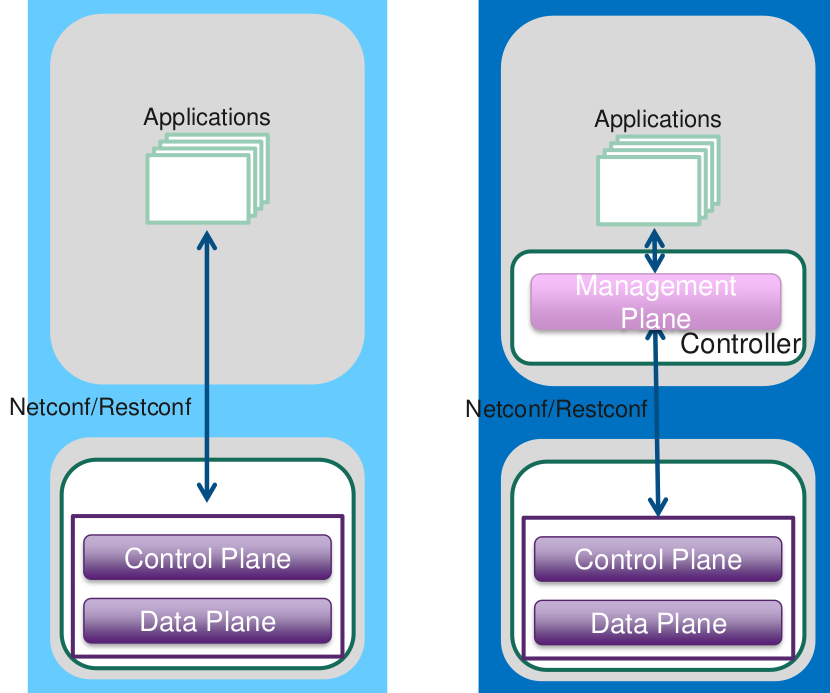
\includegraphics[width=10cm]{netconf-restconf-2in1}
	\caption{NETCONF and RESTCONF schema example}
\end{figure}

\subsubsection{Hybrid SDN, Overlay based}
\begin{itemize}
	\item Underlay Network: optimized, traditional Architecture 
	\item Overlay Network: flexible, virtual network, centralized Management Plane 
	\item Encapsulation necessary (VXLAN, NVGRE, IPSEC, \ldots) 
\end{itemize}

\begin{figure}[h]
	\centering
	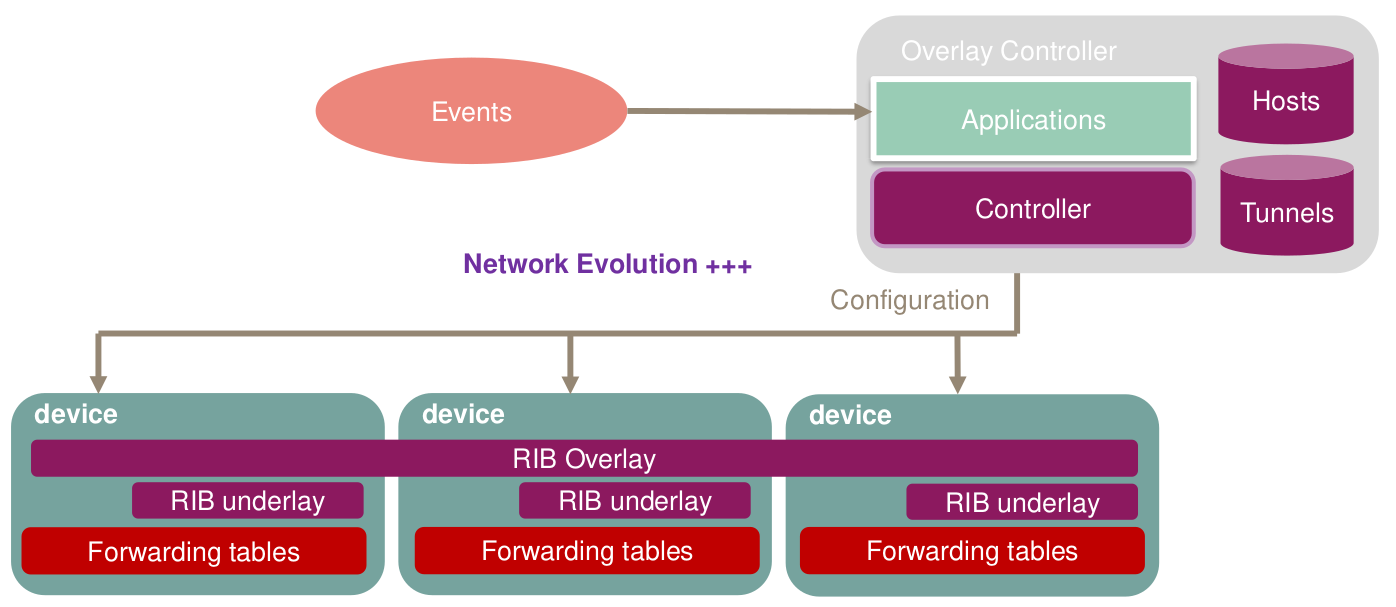
\includegraphics[width=12cm]{approach-overlay-sdn}
	\caption{Overlay SDN approach}
\end{figure}

\noindent
\textbf{Positive}
\begin{itemize}
	\item Decoupling of services and network 
		\begin{itemize}\item Service provisioning in the edge elements\end{itemize}
	\item No impact on the transport core  
\end{itemize}

\noindent
\textbf{Negative}
\begin{itemize}
	\item overhead in 
	\begin{itemize} \item Encapsulation \item Processing power \item Complexity (additional control plane) \end{itemize} 
	\item Overlay-to-physical gateways
	\item End-to-end monitoring and troubleshooting  
\end{itemize}

\begin{figure}[h]
	\centering
	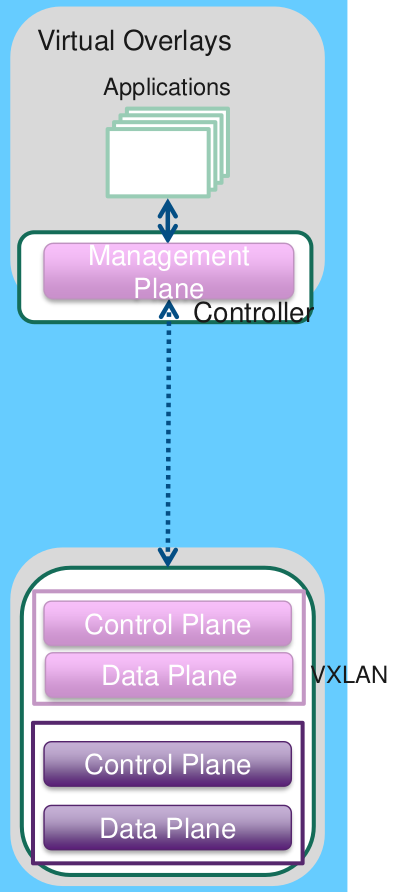
\includegraphics[width=4cm]{overlay-based-sdn}
	\caption{Overlay based schema example}
\end{figure}

\begin{figure}[h]
	\centering
	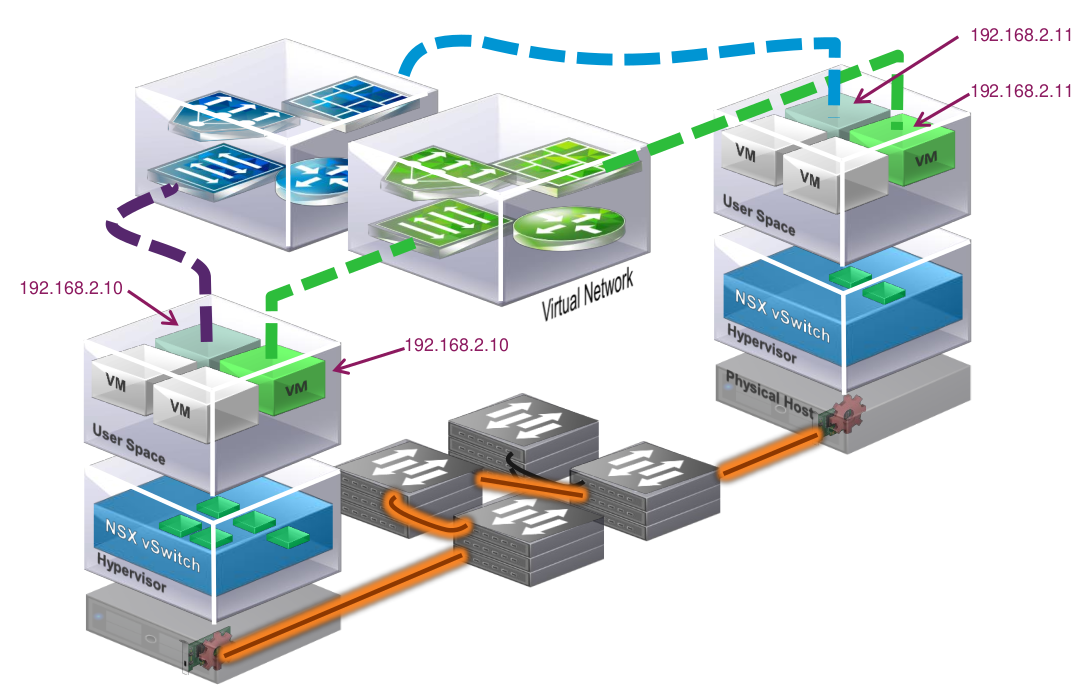
\includegraphics[width=\textwidth]{overlay-example-datacenter}
	\caption{Datacenter example of an overlay solution}
\end{figure}